\documentclass[12pt]{article}
%This Latex file is meant to be added upon and edited as seen fit by future students.
%In the interest of version control and posterity please preserve the source code of this and any other final versions with the SSC, and save any future documentation as a new version.

%Editors:
% v2017: Matthew Jasica (University of Wisconsin). Assisted by Forrest Shriver (University of Florida), Kalin Kiesling (University of Wisconsin) and Sarah Camba Lynn (Texas A&M)
%Pre-version 2017 edits that directly influenced this write-up go back at least as far as 1996, but lack a source file. Version 2017 merely marks the first time this manual was documented as a Latex file.
% v3.0 (2004): Ross Radel (Universiy of Wisconsin)
% v2.0: Hans D. Gougar (Penn State), Don Todd (Texas A&M), and Christina Plies (University of Missouri-Cambridge)
% v1.0 (1996): Richard Wenzel (University of Arizona)

%Changelog: (future editors may add on to, modify, or simplify as seen fit)
%v2017, 07-20-2017, Final push
%Updated 07-20-2017 by MJ w/ final edits and markup.
%Updated 6/04/17
%  -Include comments from K Kielsing
%Updated 5/20/17
%  -Include comments from Sarah Camba Lynn
%  -Edited title page
\usepackage[margin=1in]{geometry}
\usepackage[utf8]{inputenc}
\usepackage[colorinlistoftodos]{todonotes}
\usepackage[colorlinks=true, urlcolor=blue, linkcolor=black]{hyperref}
\usepackage{graphicx}
\usepackage{caption}
\usepackage{subcaption}
\usepackage{soul}
\usepackage{tocloft}

%\renewcommand\cftsubsecafterpnum{\vskip6pt}
\renewcommand\cftsecafterpnum{\vskip6pt}
\setlength{\parindent}{0pt}
\setlength{\parskip}{1em}


\newcommand{\redcolor}{\textcolor{red}} %Make text red to highlight changes

\begin{document}

\begin{titlepage}
\vspace*{2cm}
\centering
{\Huge\bfseries Student Conference Planning Manual\par}
%\vspace{1cm}
%\textit{\LARGE American Nuclear Society Student Sections Committee}

\vspace{2cm}
\rm{\Large Revised June 2017\par }

\vfill

\includegraphics[scale=0.75]{SSClogo.png}
\end{titlepage}

{\hypersetup{linkcolor=black}
\tableofcontents
}

\clearpage

\section{Introduction}

The next step after a bid for the ANS Student Conference is accepted by the SSC (Student Sections Committee) is to begin the planning process.
This manual was prepared by current and former student members who, collectively, possess a significant amount of experience as participants in and/or organizers of ANS student conferences.
The purpose of this manual is to preserve and document some of the best practices and lessons of previous conferences.
It is primarily addressed towards hosts who have \emph{already been selected to host the conference}, although applicants may find parts useful.
Groups wishing to submit a proposal to host a student conference should begin with reading the Student Conference Proposal Manual, also available on the website.
This Planning Manual is not meant to be a recipe or template; each student section and conference staff member must identify their own strengths and weaknesses.
The SSC encourages creativity in both the format and content of the conferences and conference proposals.
In all cases though, putting on a student conference requires a significant commitment of time and energy by the organizers.
The material presented herein may help to shorten the learning curve and optimize the use of available resources.

During the planning process, always keep in mind the purposes of the student conference.
The primary purpose of the ANS Student Conference is the professional development of both the organizers and the attendees.
This learning experience differs from the usual university classroom situation in that students are the teachers.
Student learning and development is achieved through an exchange of knowledge among peers (as is the case at any professional meeting) and through interaction with industry representatives, academia, ANS members, and ANS staff.
Additionally, the conference should demonstrate the breadth or scope of nuclear science and engineering to the attendees by bringing together the various specialties and sub-specialties emphasized at the different schools in attendance.
Finally, the conference serves to illustrate the concept and practice of a professional meeting.
Meetings serve as a vehicle for new ideas, information exchange, and the strengthening of professional relationships.
Meetings also provide an opportunity for a student to present a paper on a scientific or technical subject within a fixed time frame to a largely unknown (but sympathetic) audience.
The presentation experience is enhanced through feedback from distinguished judges representing the spectrum of the nuclear industry.

This guide is meant to be a `living' document.
To that end, conference planners are urged to communicate regularly with members of the SSC and organizers of previous conferences.
Ideas and feedback will be used to update this guide on a regular basis so that it continues to provide the kind of information planners need to put on a successful event.
ANS Headquarters Staff members, in particular the Meetings \& Exhibits Director, are also available for assistance.
Contact information for ANS Staff members can be found at the ANS website (\href{http://www.ans.org/about/staff/}{http://www.ans.org/about/staff/)}.
Alternatively, contact the SSC Chair \mbox{(\href{mailto:sscChair@gmail.com}{sscChair@gmail.com})} if there is any question about whom to contact.
Contact information for prior organizers may also be obtained from the SSC Chair.

\section{Applying to Host a Student Conference}

\subsection{Application Format}
Every year there is one Student Conference hosted by a university student section in the early spring.
The conference is planned, administered, and executed by student members of the society.
Faculty and other members of the society should be involved only in a guidance or support position.
The host university usually provides clerical and similar support.
Involvement of a nearby ANS local section, other ANS student sections, or other student organizations at the host institution in assisting with solicitation of financial support or in any support role is encouraged.
Logistic support and conference planning expertise is also available from the ANS National organization.
Applicants are strongly encouraged to take advantage of the many resources available to them through the SSC, particularly prior conference hosts.

Sections interested in submitting a proposal are strongly encouraged to notify the SSC Chair as soon as possible.
Proposal submissions are due roughly \textbf{18 months} prior to the intended conference.
The deadline for proposal submissions will be posted on the Student Conferences Page (\href{http://students.ans.org/student-conferences/}{http://students.ans.org/student-conferences/}  of the SSC website (typically this deadline will be around October 1st).
The proposal must address items in the Student Conference Proposal Manual found on the SSC website.
That manual contains more details on the proper content and format of the proposal.

Applicants must send an electronic copy of their proposal to the current SSC Chair (\href{mailto:sscChair@gmail.com}{sscChair@gmail.com}) by the stated deadline.
Proposals are limited to no more than 10 MB in size and must be submitted in PDF format.
Alternatively, the applicants may host the proposal on a web server and notify the SSC of the URL by the deadline date, although this does not eliminate the 10 MB size limit.
Hosts will then be chosen and notified during the President's Special Session during ANS Winter Meeting, again, roughly 18 months prior to the conference date.

\subsection{Selection Criteria}
A judging committee of the SSC of ANS approves by annual vote which student section will host the conference.
The judging committee is to be composed by the SSC Chair  according to rules adopted by the SSC (available for download from the SSC website).
The judging is then carried out by the committee using the Judges' Evaluation Worksheet (also available on the website) as a basis.
This worksheet is used \emph{as a guide}.
The selection committee reserves the right to consider additional features of the application should they deem it necessary in judging proposals
\href{http://students.ans.org/section-standing/}{Good standing} of applicant sections is also taken into account in judging.

Past winning proposals are \href{http://students.ans.org/student-conferences/}{available for download} on the SSC website.

\clearpage
\section{Initial Planning}

\subsection{Organization}
Establishing an organizational structure is a necessary part of the proposal, and should be well-established by the time a section is awarded the student conference.
This is so that the organizers can immediately get started with the planning of activities and solicitation of funds after the selection has been made.
It is understood that the structure may change slightly between the written proposal and the being awarded the conference based on the changing needs of the planning committee, and that not all of the people involved with the proposal writing will be a part of the planning committee.

The leadership structure has taken on many forms over the past several years.
A common form has featured two or three general Co-Chairs, each responsible for different domain, but having an equal say in key conference decisions.
However, if that structure makes it more difficult to have multiple leaders at the top without either marginalizing one or leaving people confused about who is in charge, a variation of having junior and senior Co-Chairs may be more effective.
Another option may be to simply have an appointed Assistant Chair.
Again, each situation is different, and the chosen structure should reflect the strengths and needs of the organizing committee.

The division of labor among the organizing committee varies from school to school and year to year.
However, the tasks that are performed are fairly constant.
Figure \ref{fig:OrgChart} contains a sample layout of a committee structure used for a conference.
In this example the general/ assistant chair structure is employed.
As it is beneficial to get as many people as possible involved, consider establishing additional leadership roles as the conference nears.
For example, a Professional Development Chair and Volunteer Coordinator could be appointed to perform duties that might otherwise take the time of another chair, while giving an additional student the chance to get involved.

\begin{figure}[b]
    \centering
    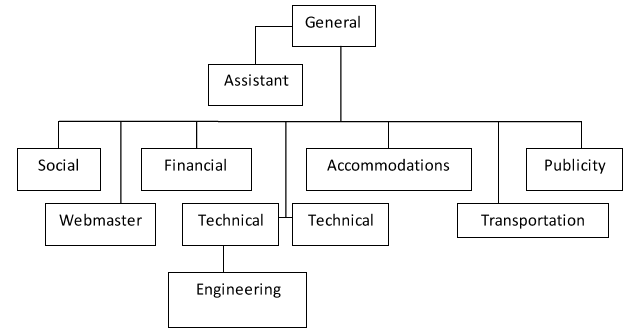
\includegraphics[width=0.6\textwidth]{OrgChart.PNG}
    \caption{Sample organization chart for a Student Conference planning committee}
    \label{fig:OrgChart}
\end{figure}

Below is a sample summary of the responsibilities of the planning committee.
This list is not exhaustive and may change based on each conference's needs.
The responsibilities listed below may be reorganized among committee members and between different committees as desired by the organizers.

\emph{General Chair(s)}
\begin{itemize}
    \item Provides overall vision and leadership and is ultimately responsible for the success of the event
    \item Sets up the major milestones and goals and directs the other Chairs to ensure that it is followed
    \item The primary interface between the conference organizers and important guests, department and college administrations, faculty, SSC, and ANS National.
    \item Primary contact for funding solicitations
    \item Master of Ceremonies for major conference events
\end{itemize}

\emph{Technical}
\begin{itemize}
    \item \textbf{The Chair of this committee should preferably be a graduate student, if possible, with prior conference experience}
    \item Organize technical sessions, workshops, panels, or other events 
    \item Oversees paper submission and review process and sets judging criteria
    \item Recruits judges and reviewers
\end{itemize}

\emph{Financial}
\begin{itemize}
    \item Manages conference funds and banking. This responsibility should be given to a member experienced with money management, likely a senior member
    \item Sets and maintains conference budget
    \item Writes financial reports for ANS National
\end{itemize}

\emph{Hospitality and Accommodations}
\begin{itemize}
    \item Coordinate with conference and lodging facilities to ensure conference and guest needs are met
    \item Sets master event schedule
    \item Organizes meals
\end{itemize}

\emph{Publicity}
\begin{itemize}
    \item Writes announcements for ANS and student members
    \item Conduct publicity campaigns with local, university, and ANS media
    \item Manages website, social media, and conference mobile app
\end{itemize}

Other components that need to be addressed include:
\begin{itemize}
    \item Managing registration and associated revenue or discounts
    \item Coordinating transportation (including to the conference city, hotels, and airports and also between conference events)
    \item Organizing student volunteers for conference staffing
    \item Organizing socials, tours and other non-technical programming
\end{itemize}

\emph{Faculty Advisor}
\begin{itemize}
    \item Advises committee on conference planning
    \item Reports to home department on progress
    \item Lobbies for department and administration support
\end{itemize}


\subsection{External Communications}
Conference committee members who will have significant contact with people outside of the conference may wish to establish  separate email addresses specifically for conference business.
Be warned that some organizations may have firewalls that prevent unknown addresses from being able to communicate via email.
In such cases committee members may wish to use their educational email address to initiate contact and then ask that the conference address be whitelisted.
Conference Chairs may establish a dedicated phone number (such as through Google Voice or a similar service) specifically for conference business if they wish to avoid publishing personal phone numbers.

\subsection{Booking Facilities}

Another task that should be accomplished soon after receiving a conference bid is booking conference facilities and reserving hotel blocks for attendees.
Discussions with these facilities should begin as early as during the proposal writing process.
The organizing committee should be prepared to enter contract negotiations as soon as they are awarded the conference.
All contracts must be reviewed and signed by ANS National.
Upon receiving a contract from a venue or vendor, forward it to the ANS Meetings Director for review, discussion, and negotiation.
Once all parties are satisfied, the ANS Executive Director will sign the contract on behalf of ANS and the Student Conference.
\emph{Do not personally, or on behalf of your student section, enter into any contracts related to the conference. 
This is to protect the organizers from any liability that they may incur from not fully meeting the terms of the contract.
\textbf{ANS National is not responsible or liable for any contracts that they have not signed.}}

\subsection{Milestone Planning}
A detailed schedule may be prepared in a milestone format detailing the events and deadlines of items from the submission of the proposal through the final accounting reports.
The milestone schedule should include, but is not limited to, information on the following:

\begin{itemize}
    \item ANS Winter and Annual Meetings (which Chairs are expected to attend). Delegates are sent to Professional Division meetings to be introduced by the prior conference Chairs and to generate interest and begin soliciting funding for the upcoming meeting. At the Annual Meeting following the conference be sure to express gratitude for any participation.
    \item Major deadlines, including registration opening and closing, summary submission (and anticipated extensions), and hotel block reservation deadlines
    \item Publication of announcements to ANS and other schools (flyers, web pate, etc.) regarding submission deadlines, hotel reservation instructions and deadlines, etc.
    \item Sending of funding solicitation letters and emails
    \item Sending of invitation letters to speakers, judges, and other special conference guests
    \item Sending of acceptance notifications to student presenters
    \item Program printing
    \item Thank you letters to sponsors and career fair attendees, speakers, judges, and other special guests
\end{itemize}

The best examples of milestone schedules can be found in the winning proposals, posted on the SSC website. 
The most recent proposals will likely contain the most relevant milestone schedules.
When scheduling milestones, one recommendation is to work backwards from the conference dates and determine external deadlines, such as those from vendors, venues, etc.
Once those are determined, all other milestones can be based on those

\subsection{Schedule of Events}
Determining the specific schedule of events is a critical framework to establish immediately after being awarded the conference, if not sooner.
The Student Conference typically run from Thursday through Saturday, taking advantage of the weekend to minimize the impact of the conference and associated travel on students' academic schedules.
Too much time during the week may discourage some students from attending (or faculty from encouraging attendance).
A successful proposal is expected to have already addressed the conference schedule and department support on at least a broad level.
A sample schedule is shown in Figure \ref{fig:Schedule}.

\begin{figure}[h]
    \centering
    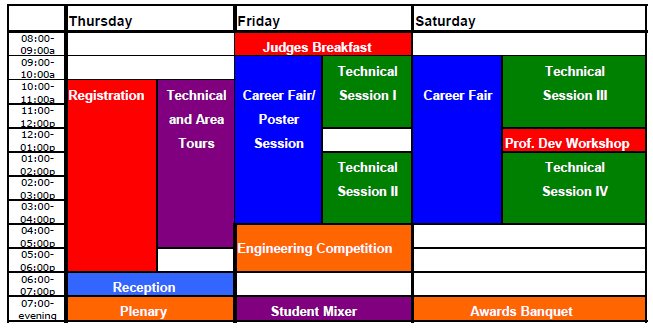
\includegraphics[width=0.8\textwidth]{SampSched.PNG}
    \caption{Sample schedule of conference events}
    \label{fig:Schedule}
\end{figure}


The organizers should consider the impact on their home department's classes and schedule.
Many students will want to take advantage of how close the conference is, or may plan to help as a volunteer at the conference.
Faculty may be asked to judge sessions or take part in plenaries and panels.
Organizers should coordinate their schedule with their department and faculty, asking them to adjust their schedules to allow for conference attendance.
Consider asking instructors to cancel classes during the conference.
This underscores how critical it is to already have support from the organizers' home department even before submitting a proposal.

\clearpage
\section{Reporting}
Reports to the Student Sections Committee and to ANS National are a required part of the planning process.
In particular, the organizers will regularly be issuing two sets of reports\---progress reports and financial reports.

Progress reports detail the activities of the planning committee, including any successes, obstacles, or subjects and perspectives that may have a bearing on future conferences. 
The proposal itself is considered the first progress report.
These reports will likely be accompanied by questions or concerns from the SSC, which are expected to be addressed in a timely manner.
All progress reports should be emailed \textbf{to the SSC Chair} (\href{mailto:sscChair@gmail.com}{sscChair@gmail.com}).
Additionally, organizers should be prepared to present their progress at the SSC meetings during all ANS Annual and Winter Meetings preceding the conference as well as the Annual Meeting immediately following the conference. 
Once the conference is closed out with ANS National, the organizers must submit a final report to the SSC Chair.
Specific content is required for this report.
The scheduling and requirements for all reports is posted on the SSC website (\href{http://students.ans.org/student-conferences/}{http://students.ans.org/student-conferences/}).

Additionally, organizers are responsible for submitting monthly financial reports via email to ANS National.
These reports must include a copy of the most recent budget with anticipated revenue and expenses, fundraising progress, and any major financial activities (e.g. placing down a deposit for the main venue).
Any significant changes from the prior month's report should be explained.
Thirty (30) days after the final date of the conference and after the payment of all bills (not including student travel assistance), the host section must prepare a final financial statement.
This statement must show the sources of all funds, disbursements (including anticipated travel assistance), and any surplus of deficit.
The records of any bank account maintained by the organizers for conference funds outside of ANS National must also be included.
This statement should be audited by the Faculty/Staff Advisor or other university personnel.
It is \emph{strongly advised} that copies of all bills and receipts be retained by the host section, at least until ANS National considers the conference closed.
All financial reports should be emailed to \textbf{the ANS Meetings Director}.

Financial reports will be kept by ANS National for a period of seven (7) years after the conference.
A copy of the financial report should be retained by the host section.

As per current federal regulations, \emph{government funds may not be applied to non-educational functions.}
Contributions from other sources may also be restricted in their use.
In such cases, the final accounting should indicate the source of funds for social events and similar functions.

\clearpage
\section{Finances}
\subsection{Financial Responsibility}
The financial responsibility for the conference lies with the host section (except where explicitly accepted by the ANS National).
Organizing the conference involves signing contracts and overseeing a budget of several hundred thousand dollars.
Depending on how the finances are handled, the conference hosts could be audited by the IRS.
Because Student Sections do not form legal entities, it is strongly advised that the host section obtains assurance of financial backing from the administration of the host university or from ANS National to avoid personal liability of the section officers or conference organizers.

The organizers should assign financial management responsibilities early in the planning process.
Responsibilities to consider include for drawing up the preliminary budget, controlling disbursements and deposits, and the financial accounting.
The organizers should determine early on how conference funds will be held.
The recommended option is banking through ANS National when allowed by host institution policy.
Another option is banking through the host institution.
Conferences have also successfully maintained secondary accounts, either through their home institution or local bank, however, \emph{it is strongly advised against maintaining a private account as the primary conference account.}

The benefits of banking through ANS are that funds are generally not restricted, the ANS Meetings Department has experience helping plan conferences (including student conferences), and that ANS has 501(c)(3) status, meaning that donations to the conference will be tax-deductible for sponsors.
The primary drawback of banking through ANS National is that large payments will take several weeks to process.
ANS can provide the organizing section with petty cash funds, which can be used to make smaller purchases without having to wait several weeks.
The use of petty cash funds must be documented in full detail in monthly reports.
Another drawback is that ANS accounting information is released only once a month, so verifying financial records at any given time can be difficult.

The benefits of banking through the host institution are that funds \emph{may} be accessed more readily, and that signing contracts with other university entities may be easier  (e.g. if dealing with university facilities or equipment).
Some universities may have meeting departments with experience organizing student conferences.
This can simplify the planning process, but these services may come with a fee.
The drawbacks of banking through the host institution are that some institutions do not automatically grant their student organizations 501(c)(3) status. 
This means that donations made to the conference may not be tax-deductible and may impact the amount sponsors are willing to donate.
Also, some institution restrict the use of funds (e.g. they may forbid the purchase of alcohol with funds held by the institution).

One more early consideration is attaining tax-exempt status.
Banking through ANS \emph{does not} guarantee tax-exempt status of the conference's purchases.
Organizers should work with ANS National and their host institution to determine how to attain tax-exempt status for any conference expenses.

\subsection{Budgeting}
The organizing committee has already created a preliminary budget in the process of applying to host the student conference.
After being awarded the conference, and monthly thereafter, the organizers should review and adjust that budget to ensure that it is an accurate reflection of the anticipated expenses, sources of funds, travel assistance, registration fees, and other finances.

\subsection{Fundraising}
There are four principal sources of funds\---ANS Professional Divisions, local sources, industry sponsors and exhibitors, and registration fees.
Registration will be discussed in a later section.

\subsubsection{ANS Professional Divisions}
It is expected that organizers to attend both the ANS Annual and Winter Meetings before their own conference and visit all of the Division Executive meetings.
The current practice is that during the Annual Meeting the previous hosts will take the upcoming hosts to each division meeting to thank the Divisions for their past participation and introduce the new hosts and their conference.
In some cases, it may not be possible for one person to attend all Division meetings, so enlist the help of several representatives to make sure every meeting is covered.
It is important to go to the Annual Meeting because by the time of the Winter Meeting, many Divisions will have already finalized their budgets.
Division Chairs should be contacted at two weeks before each national meeting to schedule time for the student conference delegates with the Division's Executive Committee.
A list of current Division Chairs and their contact information may be obtained from the prior conference Chairs.
Alternatively, contact forms for each Division Chair are available at \href{http://www.ans.org/const/divisions/}{http://www.ans.org/const/divisions/}.
Use the most recent program available from that meeting's website to find out when each Division's Executive Committee is meeting, and plan to spend about 10 to 15 minutes with each Division.
Although the conference is by no means fully planned by the time of the Annual Meeting, the organizers should be able to provide an overview of conference events, goals, and projected participation.
Consider bringing flyers with pertinent details, a copy of the fundraising prospectus, and business cards to hand out.

Many Divisions typically provide some funds for student conferences, but may provide more if a student delegate makes a personal appeal, or if the conference has a particular event closely aligned with the Division's interests.
The Divisions may also be interested in providing more than financial support.
They may be willing to help find speakers, reviewers and judges.
Be sure to highlight not only how the Divisions can help the conference, but how conference participation can benefit them.
Be aware that many Divisions will give money with specific earmarks, such as student awards or travel assistance.
 
It is particularly important to attend Division meetings at the ANS Annual Meeting immediately following the Student Conference to thank each Division.
Provide each Executive Committee and sponsor with a summary of the conference, and thank them for their support.
If a Division sponsored a student award, inform them of the winner.
Consider providing a picture of the winner and/or a copy of the winning paper.
 
\subsubsection{Local Sources}
Another source of funds are local sources, such as the host section's department or college, and ANS local sections. 
Many home institutions will want to contribute, as a successful conference also reflects well on them.
ANS local sections will often directly donate money for Student Conferences, particularly if they are geographically near the host university.
They may also provide travel assistance to nearby student sections, which will lessen travel assistance burden to the organizers.
If they cannot help out financially, local sections and programs may help the organizers find and engage other potential sponsors.
A list of Local Sections is available on the ANS website (\href{http://www.ans.org/const/local/}{http://www.ans.org/const/local/}).

\subsubsection{Sponsors and Exhibitors}
The third and largest potential source of funding is from organizations in the nuclear industry and related fields.
The best source of contacts will be the electronic databases of sponsors and contact information created by the hosts of previous conferences.
The incoming organizers should engage the prior organizers prior to fundraising as the prior organizers may also have additional information beyond contacts that may impact their conference.
This database should be updated throughout the planning process, as situations in the various companies and agencies may change from year to year.
Another excellent source of contacts will be the host institution's network.
Some programs may already have an established network of contacts or alumni for fundraising purposes.
Other faculty members may be able to personally introduce the organizers to potential sponsors.
If no prior contacts are available, many companies will have a University Relations or Recruiting Manager.
Other potential leads include the Nuclear News Buyer's Guide and U.S. Nuclear Utility.

The organizers should identify potential sponsors early in the planning process.
In addition to obvious sponsors, try to think outside the box.
Companies tangentially related to nuclear and newer, smaller companies may be interested in making themselves known at the career fair.
Some cities offer grants to assist in hosting large conferences, as they provide a boost to local businesses.
Committee members with prior relationships with potential sponsors are often the best people to initiate contact with those companies.

As soon as the conference is awarded, organizers should begin writing their fundraising prospectus.
Drafts should be sent to the SSC Chair or previous conference organizers for review.
The organizers of the next conference should be able to produce a final detailed conference prospectus and be ready to contact potential sponsors as soon as the prior conference has finished. 
\emph{\textbf{However, solicitations should be not be made to potential sponsors and exhibitors until the close of preceding conference}}.
Although details of the conference, such as specific panels, workshops, or items included with registration, are likely to change, they could still be included where appropriate to give an idea to sponsors of what to expect.
The prospectus can be provided to ANS Divisions as well as potential sponsors.
Sponsors are more likely to be supportive of organizers that demonstrate their conference planning abilities.

There are two primary methods for establishing sponsorship opportunities.
The first is to create an itemized list of sponsorship benefits and opportunities with each having an associated cost.
Sponsors can then pick and choose which benefits they would like and donate the appropriate amount.
The second is to develop multiple sponsorship levels and associate a set list of benefits and opportunities with each level.
For example, a \$25,000 donation could receive X, Y, and Z, while \$15,000 only receives X and Y. 
Benefits and opportunities include, but are not limited to, a career fair booth, advertising space, event naming rights, special awards, or promotional items provided to attendees.

Regardless of the strategy chosen, it is advisable that a career fair only option be provided.
Some companies and government agencies are limited to spending money only on recruiting, and it is important to allow these organizations to participate in the conference. 
In particular, as of 2017 the Department of Energy has adjusted their policy such that their labs and agencies cannot ``sponsor" student conferences.
However, they may still be able to financially support the conference as ``recruiters" or some other designation. 
When engaging the prior conference hosts, discuss how to appropriately engage these entities.

\subsubsection{Sponsor Relations}
Always be aware the that host section's relationship with conference sponsors directly affects future conference organizers' ability to fundraise.
If a sponsor has a negative experience, they are likely to reduce or even eliminate their sponsorship for the next conference.
On the other hand, a strong, positive experience may increase their level of sponsorship in future years.

Fundraising is primarily a \emph{chair-level responsibility}.
Except where a prior relationship has been established, contact should only be initiated by a General Chair or another senior member of the committee.
Not only does this person represent the ANS Student Conference to the industry, but they need to have the authority to make decisions that impact the entire conference.
Be prepared to negotiate with all sponsors and donors.
\emph{Reasonable} special requests by each company should be considered.
Treat all sponsors and exhibitors fairly.
If one sponsor is granted a special request, any similar special request by another sponsor should also be granted.
However, do not be afraid to say no to unreasonable demands, even if it will upset a sponsor.
There is no right or wrong way to handle special requests from sponsors.
If there is a question of whether or not a request is reasonable or how to handle an uncomfortable situation, advice can always be solicited from prior Chairs or the ANS Meetings Director.

The single, most important key to establishing a positive sponsor relationship is to show the sponsors appreciation for their donation.
Send thank you notes or emails to every sponsor.
If a company sponsored a specific event, consider sending them pictures of the event.
If they did not sponsor a specific event, general conference pictures may be sent instead.

\subsection{Travel Assistance}
A major expense is the payment of travel assistance to student attendees.
Many methods have been used to determine the amount awarded, but the critical thing is to ensure a fair and transparent distribution, whether it is based on distance traveled, mode of transportation, or any other metric.
Travel assistance should be provided \emph{to students only}.
It is left to the discretion of the organizers what specifically is eligible, but typically any travel-related expenses to and from the conference site are eligible, including parking at the hotel and/or airport, airfare, gasoline, taxi or rideshares to/from an airport.
Non-travel expenses, including lodging, food, and registration are typically  ineligible.
Some institutions may provide subsidies to their own students.
The organizers must decide in advance if and how to provide additional subsidies to students from these institutions.
Some conferences have had the policy to only provide assistance to students staying at an official conference hotel.
This has been done to reduce attrition payments owed to the hotels that would result from not filling the rooms contracted by the organizers.
If attrition is not a concern, organizers may choose to not make this a requirement.
Whatever policy is decided, \textbf{all attendees should be made aware of all travel assistance policies and procedures well before the conference.}

When at all possible, requests for assistance should be made by student sections rather than individuals. 
All requirements and procedures for assistance should be made known to attendees well before the conference.
The travel assistance should be distributed \emph{after} all other expenses have been settled.
If banking is done through ANS, notify ANS of the final amounts to be disbursed to each section, and ANS will transfer this money from the conference bank account before closing out the meeting.
ANS will not write checks to individuals unless the individual does not have a home student section.
The assistance should be given in a lump sum to each student section.
The student section will then be responsible for distributing the funds among its students.

\subsection{Seed Money \& Surplus Funds}
Early in the planning process, ANS National can provide the organizers with \$5000 of seed money for early down payments and expenses.
This is essentially an interest-free loan.
It is expected that this seed money will be paid back to ANS National following the payment of all conference expenses.
This should be clearly indicated in the final financial report.

Seventy-five (75) percent of any net revenue, accounting for travel assistance and repayment of seed money, is retained by the host section.
The remaining twenty-five (25) percent of surplus funds is due to ANS National.
These funds are used to offset the cost of services rendered to the organizers, 
including ANS personnel time and resources.
It is suggested that surplus funds be used for local educational purposes, such as support for future student section functions, conference attendance, outreach materials, etc.
Some host sections have set up an endowment with the surplus funds for future section activities.
Rarely, the surplus funds may exceed what the host section feels is necessary to support themselves.
In the past, excess funds have been donated to the SSC (under the care of the Young Members Group) to support ANS student members on a national level, or given directly to the next student conference.
The decision to do this lies solely with the organizers.
Restrictions on the funds may be placed by the organizers.

\clearpage
\section{Registration}
Online registration for the conference is provided by ANS National.
The registration form will be created and hosted by ANS.
Contact the ANS Registrar (\href{mailto:registrar@ans.org}{registrar@ans.org}) to facilitate the creation of the registration form.
The conference organizers should provide the registrar with the necessary fields and event information no later than mid-September so that registration can be live before the Winter Meeting.
This includes details for all workshops, tours, or other events requiring advance registration, such as time and capacity.
Any sign up deadlines for any event should also be included.
ANS also has the ability to create waitlists for events as requested by the organizers.
This allows all payments to be handled through ANS National, which is especially convenient if conference hosts are banking through National.
ANS will be able to send monthly reports (or more frequently, as requested) to the organizers, including contact information, meal and other selections, and event participation and waitlists.
Once the page has been set up, the link should be advertised by the organizers.
Possible advertisement modes include conference social media, website posting, and SSC or ANS National announcements.
Additionally, a separate form can be set up by the organizers to help students traveling alone find a roommate and cut lodging cost.

To help meet the cost of the conference, and more importantly, to create a sense of commitment, a small registration fee is usually charged.
At the discretion of the organizers, special guests, speakers, judges, volunteers, etc.\ may be exempt or receive a discount for this fee.
The ANS system is flexible and able to adapt to the financial and registration needs of the organizers.
Although it is customary to award sponsors and significant speakers some complementary registrations or discounts, \emph{be conscious of how many registration discounts are given out.}
The purpose of the higher cost of the professional registration is to minimize the cost of the conference to the students.
Any money that is given to professionals is money that cannot be spent on the students.
With this purpose in mind, some professionals may understand the registration fee structure.
Others may be upset about the cost, but generally become understanding about this.

Priority for tours, workshops, and other special events should be given to visiting students.
Policies regarding the participation of students of the host institution in events with limited space are at the discretion of the organizers
One option is to ask students from the host institution to wait to register until closer to the conference.

Plots of the total registration number versus date are shown in Figure \ref{fig:Reg} for the 2012 Student Conference (held April 12-15) and 2016 Student Conference (held March 31-Apr 3).
They show the difficulty that can be had in predicting attendance for the conference.
It is recommended that the early registration deadline is after the notification of acceptance of summaries.
Students may wait until they know that their summaries are accepted to register.

Historically, other options besides hosting registration through ANS National have been utilized.
Internet services such as PayPal have been used for internet-based registration payments.
The drawbacks are that these may incur a fee for each payment, and do rely on an external vendor for handling a significant portion of conference finances.
It is strongly recommended that organizers take advantage of the registration services ANS has to offer.

\begin{figure}[h!]
    \centering
    \begin{subfigure}[b]{0.75\textwidth}
        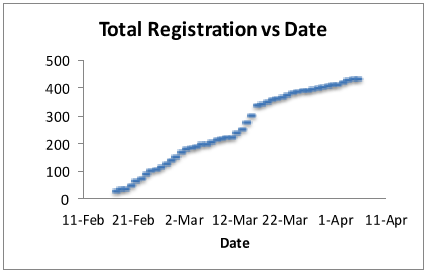
\includegraphics[width=\textwidth]{Reg2012.PNG}
    \end{subfigure}
    
    \begin{subfigure}[b]{0.75\textwidth}
        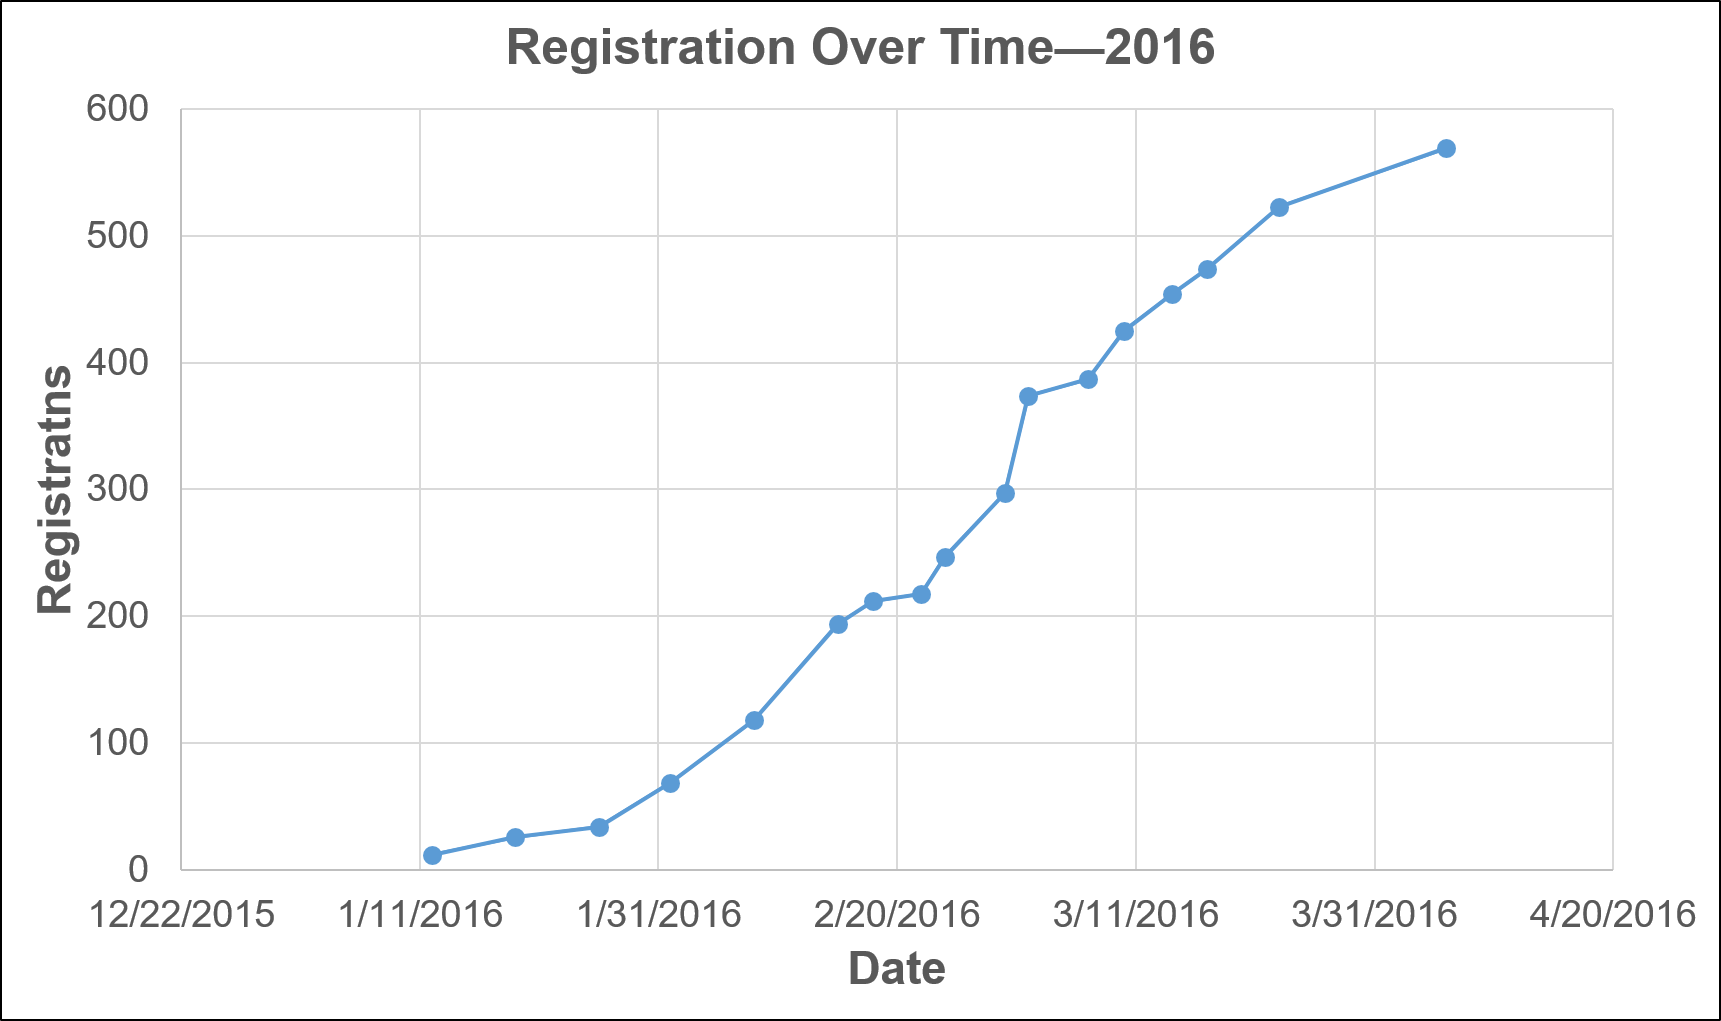
\includegraphics[width=\textwidth]{Reg2016.png}
    \end{subfigure}
    
    \caption{Registration trends from 2012 (top) and 2016 (bottom)}
    \label{fig:Reg}
\end{figure}



\clearpage
\section{Program}

\subsection{Technical Program}
\subsubsection{Summaries and Formats}
Presentations at the conference are to be authored and presented by current students only.
The students need not be student members of the society, nor majoring in nuclear science and engineering.
Their papers should, however, concern a subject related to nuclear science and engineering.
This subject might concern the student's thesis research (including a progress report), a design project, a slightly unusual laboratory project, or even an off-shoot of material in a book.
In some cases (such as a senior design project) multiple students may collaborate on the same project.
Students who contributed significantly, even if they are not a part of the presentation, should be listed as co-authors.
The problem may have been suggested by a faculty member who has provided guidance, but the translation of the idea into a completed project should be carried out by the student(s).
Any faculty significantly involved in the project should be listed as co-authors (following the participating students).

There are only two formal portions of a presentation, the written summary and the presentation itself (either as a poster or podium presentation).
The submission of summaries prior to the conference by every student presenter is required.
It should be understood that the summary is the only portion of the presentation to be published.
It is also the only written submission for the conference; there is no full-length paper submission.
\emph{Please note that summaries are not simply abstracts.}
It is a ``stand-alone" document rather than an introduction to a full-length paper.
Therefore, special care should be exercised, ensuring that it is complete and accurate.
A good summary will answer the following:

\begin{itemize}
    \item What was done? (Introduction)
    \item Why was it done? (Background Information)
    \item How was it done? (Experiment/ Procedure)
    \item What was found? (Results, Analysis, \& Conclusion)
\end{itemize}

Summaries should be typed and submitted digitally through the Electronic Paper Submission and Review (EPSR) system hosted through the ANS website.
The organizers will need to work with ANS National to set up the submission /site.
Please use the {ANS Transactions} used for ANS professional meetings.
Submissions should be submitted as \textbf{PDF format only}. 
Guidelines and a template can be found at \href{http://www.ans.org/pubs/transactions/}{http://www.ans.org/pubs/transactions/}.

The first Call for Summaries and submission site should be ready around the same time that registration opens (around the ANS Winter Meeting).
The SSC can provide a sample Call for Summaries.
At the same time, the organizers will want to put out a Call for Reviewers and Judges to recruit these volunteers.
Again, the ANS Divisions are excellent sources for these.
Reviewers will comment and make suggestions on submissions, while judges will attend the conference to judge student presentations.
Be sure to consider the following when setting a submission date:
\begin{itemize}
	\item It is customary to postpone the submission date by one or two weeks to allow students who may be a little late with their papers the opportunity to submit.
    \item Allow at least 1-1.5 weeks for reviewers to review papers. Remember that these are professionals who are volunteering their time. The organizers should be prepared to review any unreviewed papers by the end of the review period within the best of their abilities. It is best to have professionals or senior graduate students familiar with the field review papers. However, this is not always possible in last-minute situations. To address this, it is helpful to have a few willing and experienced students be on call to do last-minute reviews if the organizers do not feel comfortable reviewing these themselves. Gentle reminders to reviewers can help minimize this.
    \item Most reviewers will only reasonably review around 5 papers on average. Some may be able to review more. It is recommended that each paper received a minimum of 3 reviews, so be sure to find enough reviewers to accommodate the anticipated number of summaries.
    \item Again, many students will wait to register and book a room until they know if their paper has been accepted. Plan to have all submissions reviewed and returned to students before the Early Registration deadline.
\end{itemize}

It is recommended that the final accepted summaries be reproduced as received and issued as conference transactions, made available to students after the conference.
Possible distribution formats may include a USB stick or making available online to registrants.
Conference Transactions should also be distributed to the host institutions, the SSC Chair, ANS Headquarters, and contributors, if asked.
As of 2017, there is no formal record of student conference transactions maintained by ANS National as it does with other professional meetings.

\subsubsection{Oral and Poster Presentations}
Students have had the option to designate their summary as either a poster or oral presentation.
It is at the organizers' discretion to determine whether a submission is more appropriate for a poster or oral presentation.
In general, the organizers may rely on recommendations by reviewers to switch a submitted poster to an oral presentation or vice-versa. If it is recommended that a submission is switched, the authoring student should be informed as soon as possible.
In either case, the student presenter should make an effort to present the material in a manner that is understandable to fellow students.

Oral presentations are typically divided into sessions organized by field.
These fields generally follow the ANS Professional Divisions, although some variation exists at the discretion of the organizers.
The typical time allotment for oral presentations is 15-20 minutes for the presentation followed by 5 minutes for Q\&A.
Assigning a student or professional to act as a moderator in each session has proved an effective way to ensure presenters stay within time limits, and provides someone to introduce and assist with technical problems should they arise.

Poster presentations are set up early in the conference for conference attendees to view.
One afternoon is designated for the formal session where presenters are required to stand by their poster and answer questions from visitors and poster judges.
Generally, students should not be expected to be present at their posters for more than 1.5 hours.
This is at the discretion of the organizers, but bear in mind the comfort of the students and professionals as this room can become very warm.
It is up to the organizers to determine how many posters they can accept and how large each poster can be.
Be careful to allow for sufficient space in the poster session venue to allow presenters and visitors enough space to move through the session.

The organizers should provide proper equipment to allow students to give their presentations.
For oral presentations this includes A/V equipment such as projectors and screens or monitors, laptop computers to host the presentations, along with accessories such as laser pointers.
For poster presentations this includes poster boards and tacks.
\emph{Communicate clearly to the students exactly what will and will not be provided, and any rules for presentations.}

\subsubsection{Judging}
If the presentations are judged, the judges should use the opportunity to enhance the learning experience for every presenter.
The opportunity for receiving constructive criticism is more important than being selected as an award winner.
The following guidelines are offered:

\begin{enumerate}
    \item Both technical content and manner of presentation should be judged. Although they need not present the results of original research, the presenters are expected to inform and/or educate the audience about a selected technical topic.
    \item The problem of balancing undergraduate papers against Ph.D dissertations is one of the most difficult tasks facing judges. Therefore, they should be made aware of judging criteria by the conference organizers. A rubric should be drawn up by the organizers. Presentation guidelines should be made available to presenters before the conference. Students should be asked to identify themselves as undergraduates or graduates to the judges at the start of their talk.
    \item At least two (preferably three) judges should judge each technical session. If possible, all sessions within a particular field should be judged by the same judges for consistency (although this may be impractical for some of the larger fields). Judges may be drawn from universities, industry, government laboratories, and other similar facilities. Professors should not be in a position to evaluate their own students. Again, the ANS Divisions are a great source of judges. In a pinch, experienced graduate students may also be qualified to judge talks in their fields.
    \item Honoraria, travel subsidies, and food allowance should not be paid to judges, though they should be thanked for volunteering their time.
    \item The final tabulation of scores and awarding of ``best in track" may be performed by the organizers. In this case, judges should submit their review forms to a common location following the conclusion of the final presentation in their session. This helps to normalize judging between sessions in the same track that may have different judges. Another option has been for the judges to collaborate and nominate among themselves a ``best in track".
    \item After the judging and award process is complete, the judges' critiques should be made available to each presenter in the session. The judges may or may not sign the critiques according to their preference.
\end{enumerate}

\subsubsection{Awards}
The awarding of prizes or mementos to students who have given outstanding papers is encouraged. The following guidelines are recommended:
\begin{enumerate}
    \item The competition for prizes is not the primary purpose of the technical program. The emphasis is the student presentations. Nonetheless, the incentive of an award sponsored by an ANS Professional Division has been used to boost student submissions and awareness of tracks with fewer submissions. Organizers should work with each individual division to determine what is appropriate for each track.
    \item Competition among schools should be discouraged. The experience and possible award should be a personal or group effort and achievement, not an institutional one.
    \item Awards for best presentation in technical tracks should not be given out to students of the host institution as it is common for the majority of judges to be affiliated with the host institution, which can introduce bias. That is not to say that students who perform particularly well should not be recognized by their school at a later time, but awards should only be given to students from other schools.
    \item The final banquet is the preferred time and place for the awards presentation.
    \item If awards are given for different tracks then they should be awarded for each track, even if the awards are not equal. The organizers should be prepared to award more than one prize in a session for instances in which judges cannot make a clear decision between multiple equally good papers. The recommended name for such awards is ``Best Presentation in the X Track".
    \item As stated before, there is a significant difference in judging an advanced graduate student presentation versus an undergraduate one. In tracks with significant participation consider awarding both a ``best undergraduate" and ``best graduate" award. 
    \item There may be special best presentation awards directly sponsored by ANS Professional Divisions or other entities; care should be taken to properly select and acknowledge the awards. Typically these awards are monetary, where some of a Division's contribution is earmarked for this purpose at their request. Typically these earmarks are not equal between all Divisions, nor does each Division earmark money for awards. These earmarks should be adhered to as much as possible, despite their differences. If a sponsoring Division member is present they should be given the opportunity to present the award.
    \item The monetary or real value of the awards should be small (exempting award amounts specified by ANS Professional Divisions). Personalized mementos should also be considered. Imaginative prizes in the past have included framed historic reproductions, Lichtenberg figures, and etched glass mugs. 
    \item In addition to judging presentations at the conference, conferences have also given awards for six ``Best Overall Paper", based solely on the reviews of the written summaries. The winners of this award have been invited to publish full-length articles in a special issue of the ANS Journals, a set of prestigious peer-reviewed journals in the field of nuclear and radiation science and technology. This recognition and publication opportunity has been positively received by both the students and the journals, and is strongly recommended that future conferences continue this special award. Organizers should coordinate the publication efforts with the SSC and award winners following the conference. The review process and publication will be handled by the SSC-designated special issue editor.
\end{enumerate}

\subsection{Speakers, Panels, \& Workshops}
In addition to the technical events, the student conference is an excellent venue for showcasing leaders across multiple fields within the nuclear industry.
These speaking opportunities may take the form of a daytime plenary, a panel of speakers, leading a workshop, or a dinner keynote speaker.
Speakers should be contacted as soon as possible in the planning process.
The current ANS President is usually willing and able to address the conference at one of the dinners.
Contact ANS National to make arrangements.
Any high-profile individual in the nuclear industry is an appropriate choice.
Distinguished speakers should receive a personal invitation from the Conference Chairs.

The most coveted speaking opportunities are the conference dinners when the highest audience attendances are anticipated.
Although speaking opportunities may be tied to sponsorships, the organizers may wish to invite someone from an organization unable to sponsor such an event (such as government representatives).
In such cases it is acceptable to invite the speaker for a different opportunity not tied to sponsorship, but inform the speaker that they may also be invited to speak at another time depending on if that opportunity becomes available.
Organizers should not expect to provide every speaker with complementary registration, as is sometimes done at professional meetings.
Again, the Student Conference is primarily for the professional development of the students, and any money spent on professionals is money that is not able to be applied towards keeping costs down for students.
However, organizers may wish to provide special speakers with complementary registration or other benefits at their discretion.
The faculty advisor or past conference Chairs can help determine who it is appropriate to specially accommodate. 

Workshops provide an opportunity for interactive classes covering areas such as technical subjects, outreach ideas, or professional development topics. 
Leading workshops is not only reserved for professionals, student leaders may also be considered based on their expertise or experience in a particular area. 
Panels are an opportunity to bring in multiple experts and perspectives on a topic and may include both speaker presentations and audience participation.
It is expected that a list of potential workshops and panels be prepared during the proposal process.
However, it is not uncommon to receive requests from sponsors or ANS Professional Divisions and Committees for time and space to put on additional events.
What is accommodated is at the discretion of the organizers, although more weight should be given to requests that come from within ANS National.
Remember that the focus of the program should be on the student presentations; however, it is acceptable for on-site workshops and panels to overlap with student presentations.

\subsection{Tours}
Technical and non-technical tours are typically offered on the first day of the conference for external educational or social experiences.
These tours range in topics, and often take advantage of local nuclear industry that is within driving distance, show off the host university’s research facilities, or guide attendees through significant cultural landmarks. 
As the conference approaches, be cognizant of tour registrations, waitlists, and deadlines, especially for tours that have to lock in attendee lists in advance (such as nuclear power plants or government laboratories).
It is not expected to have enough space on the tours for all registered conference attendees. 


\subsection{Social Events}
Students will learn as much, or more, during informal discussions with other conference attendees as they will from formal sessions.
Carefully designed socials are valuable student networking opportunities with both professionals and peers.
Many professional relationships have been built at ANS student socials.
When planning a social it is worth keeping in mind the following considerations:
\begin{enumerate}
    \item First, socials are \emph{not} the focus of the conference, and are by no means mandatory. If funding does not allow for it, socials (or food and beverage tabs at such events) should be among the first items cut.
    \item Although a non-technical or after-hours event, any social is still considered an official conference event. The next morning's conference events should be considered when deciding on an end time for the social. End times should allow for students to get 8 hours of sleep before the first morning events. This also means that all actions at the social reflect not only upon the conference and conference organizers, but also upon ANS National. Consider carefully any liability issues associated with any planned event.
    \item Logistics to consider are the capacity of the venue, food and beverage minimums, rental costs, the transportation for getting there, and whether that space will be shared with other patrons.
    \item If a social featuring alcohol is hosted, an non-alcoholic alternative event \emph{must} be provided, even if underage students are allowed at the venue. Possible ideas include ice skating, sporting event, trivia or game night, or mixer at a local cultural center such as museum.
\end{enumerate}


\clearpage
\section{Hospitality}
\subsection{Facilities}
As much of the siting of conference venues and hotels has been discussed in the Proposal Manual, it will not be repeated here.
One thing to pay attention to when contracting hotel blocks is the number of contracted rooms and nights.
While most hotels will reserve a room block for the conference in advance, many will require payment, known as ``attrition", if a certain percentage of the contracted room-nights is not booked to make up for lost revenue.
Consult with previous conference organizers and the ANS Meetings Director for appropriate numbers.
As one incentive to reduce the risk of attrition, some organizers have made staying in the conference hotel a requirement for receiving travel assistance.
As part of the contract, the hotels may offer a limited number of free upgrades for VIPs.
Consider awarding these to keynote speakers, the ANS President, or top sponsor representatives.
Confirm with these guests (particularly government representatives) whether or not they can accept any upgrades.
Due to the demanding nature of the position, the conference Chairs may also want to ask for a guest room set aside for their own use (showering or resting) during the conference weekend.

\subsection{Transportation}
Do not underestimate the transportation needs and expenses for the conference (a typical pitfall of proposals).
Although adequate transportation does not typically stand out after the conference, attendees will remember transportation delays that led to them being late to meals or events.
Transportation needs typically fall into three categories:
\begin{enumerate}
    \item Transportation between airports and the conference hotel(s)
    \item Transportation between conference events
    \item Transportation between the hotel(s) and the conference facilities (if applicable)
\end{enumerate}

The majority of students will travel by air to the conference venue and need some mode of transportation to reach the conference hotel(s).
If possible and within the budget, well-organized transport to the conference can make a great first impression.
If the conference hotel(s) are near a major airport, a variety of options may be available, including hotel shuttle, private shuttles, public transit, taxi, and ridesharing apps.
It may not be necessary to provide organized transportation to the hotel(s) if options are readily available and clear instructions are provided.
Organizers should not rely solely on hotel shuttles, as they may not be able to provide the capacity or frequency needed to accommodate all attendees.
If travel between the airport and hotel is not convenient or far away, organized transportation,  may be necessary.
Some attendees may choose to fly into some airport other than that designated by the organizers. 
It may not be reasonable to organize transportation for every contingency, but it would be wise to provide recommendations for obvious alternatives.
For groups that are driving to the hotels, consider where attendees can park, whether it is on-site or in a parking garage (pay parking is acceptable).
Although the conference may not be organizing and paying immediately for all transportation to the host city, these expenses may still manifest themselves in the form of travel assistance.

Travel between events is generally more straightforward, particularly for events such as tours that have a limited capacity and rely on a fixed number of shuttles and trips.
However, transportation for larger events, such as a dinner, that involve multiple shuttles and trips requires more coordination.
Plan to be able to transport every attendee to the venue, and schedule shuttles accordingly, starting as early as necessary.
Assume that delays will occur due to loading, unloading, and traffic.
Even if walking or public transit alternatives are available, consider that many attendees may be wearing uncomfortable walking shoes and that walking may not be a viable option.
A good rule of thumb is that shuttle transportation should be organized if the distance to between sites is further than $1/3$ mile.

Similar considerations apply if the conference hotel and facilities are not in the same location.
Shuttles should run during the entirety of the day, as attendees may wish to return to their hotels during the day.
Extra transportation will be required at the start of the day and before major events, such as dinners.

In all cases, \emph{communication with attendees about their schedules and the organizers' expectations is key for smooth travels.}

\subsection{Staffing}
Staffing is mostly covered in the Proposal Manual, but a few more points are worth noting here.
Organizers will want to start advertising the conference and need for volunteers early on in the planning process.
Not only will each individual session or event need a volunteer, but additional volunteers to assist with setup, registration, and assisting visitors with transportation are also required.
\emph{It is always better to be overstaffed than understaffed.}
Past Chairs have had success with utilizing one or two volunteers (outside of the committee) devoted exclusively to running errands and being the point of contact for the Chairs for any hiccups or problems.
Again, early and clear communication with the volunteers of their duties, who they report to, and the organizers' expectations is essential for a smooth conference.

\clearpage
\section{Publicity}
\subsection{Electronic Media}
An integral part of hosting a conference is the dissemination of information about the conference.
Aggressive use of a combination of email, website, and social media is encouraged.
The best option for reaching out to ANS members is emails sent through ANS National.
They will be able to assist with any design and wording, and can send the announcement to any subset of ANS members, however they cannot send any attachments besides embedded URLs.
A minimum of two weeks notice is necessary to send these out.
The current Meetings \& Exhibits Director can advise who the appropriate contact for these blast messages is.

Another option for mass communication to student members is through the SSC Chair. 
All messages should include relevant deadlines, the conference website URL, and contact information.
%Attachments such as flyers can be included in these messages.
The organizers may also wish to communicate directly with registered attendees using email addresses collected during the registration process.
Any attachments should be converted to PDF format for cross-platform compatibility.
It is important to communicate expectations (such as behavior and dress code) for speakers, judges, and general attendees in advance of the conference, as this may be the first conference for many student attendees.

A conference website is one of the most efficient means of communicating information such as deadlines, announcements, sponsor \& recruiting information, and travel information.
For many professionals and students this will be their first impression of the conference!
The website is also a good place to host forms for attendees other than registration.
Each year's conference organizers are responsible for establishing and maintaining their own website
Social media, Facebook and Twitter in particular, have been used to great effect to communicate realtime updates both leading up to and during the conference.
The ANS National social media is another good platform for advertising the conference, along with the hashtag \#ANSMeeting.

\subsection{Conference Mobile App}
Another trend since 2014 is the use of a conference mobile app where attendees have access to the conference schedule, can make their own schedule, and receive realtime updates.
Prior conferences have taken advantages of ANS National's relationship with app-building companies for a discounted fee. 
The organizers will work directly with the app developer to build the app.
Consult with the ANS Meeting Organizer for available options.
Particularly ambitious or talented organizers may be able to develop their own app in-house.
In either case, make sure all necessary information is communicated well in advance of the conference date so that the developers have time to secure the necessary permissions to publish the app on all major app stores for download.

\subsection{Print Media}
Conferences should be publicized in print as well.
All ANS student members have access to \textit{Nuclear News}, in which a calendar of events is listed.
\textit{ANS News} also contains information about upcoming events.
A copy of advertisements and items to appear in the publication should be forwarded to the Editors of these publications.
The advertisement should include: conference title, dates, name of host institution, location, and names, phone numbers, and email addresses of the conference Chairs. 
Organizers are also encouraged to communicate with local news outlets.
Following the conference, a concise report and high-resolution photographs from the conference should be forwarded to the Editors of \textit{Nuclear News} and \textit{ANS News}.
Be sure to caption and identify any persons appearing in the pictures.

\subsection{Branding}
A visual brand helps establish a quick association with the conference and its theme.
The use of a conference-specific brand will help to distinguish the conference media from others, lending a more professional appearance.
Early in the planning process the organizers should contact the ANS National Marketing Department regarding the design of conference logos and graphics.
These graphics can then be used to publicize the conference, including in letterhead, flyers, electronic media, registration items, conference program and more. 
Business cards are recommended for the conference Chairs and any other committee members who will be dealing with a great number of people.
\emph{Any logos or graphics used for the conference must be approved by ANS, as does any use of the ANS logo.}
ANS National can also assist with designing and printing many conference items such as conference programs, name tags, and event signs for a small fee.
Contact ANS National early enough to make sure that all printing deadlines can be met.

\clearpage
\section{Liability}
The importance of discussing liability for conference functions with ANS National cannot be overstated.
Once again, \emph{all contracts should be reviewed and signed by ANS National.}
By having ANS National signing these, the associated liability falls upon them and not upon the conference.
Given ANS's personnel and financial resources, this is a much more manageable situation than being held personally liable for any incidents.
Before finalizing any events (socials in particular), make sure that all liability issues are completely addressed. 
In addition to being the best resource for any liability questions or concerns, ANS can help the organizers draw up waivers or contracts as needed.
Although alcohol is the most notorious of these, it is not the only source of liability.
Things to consider include, but are not limited to:
\begin{itemize}
    \item \textbf{Financial} If the conference is unable to pay a contracted amount to a vendor, who is responsible for fulfilling that payment and how? What steps are necessary to avoid this situation?
    \item \textbf{Hotel Attrition} Does the hotel require that a minimum number of rooms and nights be paid for? How will the organizers ensure that minimum is met?
    \item \textbf{Dining} Who assumes liability for food-borne or similar dining-related illness? How will food and beverage minimums be ensured?
    \item \textbf{Personal Injury} Does any event have the capacity for serious injury? If so, are waivers required and who assumes fault for any injury?
    \item \textbf{Transportation} Who is responsible for damages to person or property in the event of an accident?
    \item \textbf{Alcohol} Who is responsible for ensuring only of-age attendees are present and consuming alcohol? Who is responsible in the event of underage consumption or police involvement?
\end{itemize}

\clearpage

\section{Post-Conference Responsibilities}
After the conference is over, a couple of final responsibilities remain. Many of these are covered more thoroughly earlier in this manual, but are included here as a concise final reminder.

\begin{itemize}
    \item Settle all outstanding payments to outside vendors and venues.
    \item Collect travel assistance information and determine how much to distribute to each student section. Organizers should coordinate with ANS National to distribute this.
    \item Distribute any outstanding student awards.
    \item Submit a final financial report to ANS National and settle any final transactions between the student section and ANS National.
    \item Submit a final report to the SSC according to the guidelines posted on the SSC website.
    \item Coordinate the publishing of outstanding student papers with the ANS journals and authors.
    \item Make student summaries available to attendees.
    \item Forward a summary of the conference to the Editors of \textit{Nuclear News} and \textit{ANS News}.
    \item Attend the proceeding Annual Meeting to give a summary report to the Professional Divisions and introduce the new Chairs.
    \item Finally, thank you letters should be sent to everyone who helped make the conference a success, including sponsors and recruiters, ANS Professional Divisions, speakers, the organizers' Department Head and other key personnel. 
\end{itemize}

\end{document}
